%%%%%%%%%%%%%%%%%%%%%%%%%%%%%%%%%%%%%%%%%
% Short Three-Column Newsletter
% LaTeX Template
% Version 1.0 (11/9/13)
%
% Original author:
% Frits Wenneker (http://www.howtotex.com) 
% With extensive modifications by:
% Vel (vel@latextemplates.com)
% 
% This template has been downloaded from:
% http://www.LaTeXTemplates.com
%
% License:
% CC BY-NC-SA 3.0 (http://creativecommons.org/licenses/by-nc-sa/3.0/)
%
%%%%%%%%%%%%%%%%%%%%%%%%%%%%%%%%%%%%%%%%%

%----------------------------------------------------------------------------------------
%	PACKAGES AND DOCUMENT CONFIGURATIONS
%----------------------------------------------------------------------------------------

\documentclass[10pt,a4paper]{article} % Paper type (a4paper, usletter or legal) and font size (10, 11 or 12)

\setlength\topmargin{-48pt} % Top margin
\setlength\headheight{0pt} % Header height
\setlength\textwidth{7.0in} % Text width
\setlength\textheight{9.5in} % Text height
\setlength\oddsidemargin{-30pt} % Left margin
\setlength\evensidemargin{-30pt} % Left margin (even pages) - only relevant with 'twoside' article option

\usepackage{charter} % Charter font for main content

\frenchspacing % Reduces space after periods to make text more compact for a three-column layout

\usepackage{graphicx} % Required for including images
\usepackage{amssymb,amsmath} % Math packages
\usepackage{multicol} % Required for the three-column layout of the document
\usepackage{url} % Clickable links
\usepackage{enumitem} % Reduces the amount of space within and between lists with [noitemsep,nolistsep]
\usepackage{marvosym} % Required for the use of symbols
\usepackage{wrapfig} % Allows wrapping text around figures
\usepackage[T1]{fontenc} % Use 8-bit encoding that has 256 glyphs
\usepackage{datetime} % Required for defining a custom date style
\newdateformat{mydate}{\monthname[\THEMONTH] \THEYEAR} % Set a custom date format
\usepackage[pdfpagemode=FullScreen, colorlinks=false]{hyperref} % Link colors and PDF behavior in Acrobat
\usepackage{fancyhdr} % Required to define custom headers/footers
\pagestyle{fancy} % Enables the custom headers/footers for all pages following this

%-----------------------------------------------------------
% Header and footer
\lfoot{\footnotesize % Left footer containing newsletter contact information
	Studying in four different countries during my Master Degree\\
	\Mundus\ \href{https://github.com/stefanos1316/my_blog/index.com}{my\_blog/index.com} \quad
	\Telefon\ Not available yet \quad
	\Letter\ \href{mailto:sgeorgiou@aueb.gr}{sgeorgiou@aueb.gr}
}


\cfoot{} % Empty center footer

\rfoot{\footnotesize ~\\ Page \thepage} % Right footer - page counter

\renewcommand{\headrulewidth}{0.0pt} % No horizontal rule for the header
\renewcommand{\footrulewidth}{0.4pt} % Horizontal rule separating the footer from the document
%-----------------------------------------------------------

%-----------------------------------------------------------
% Define separators
\newcommand{\HorRule}[1]{\noindent\rule{\linewidth}{#1}} % Creates a horizontal rule
\newcommand{\SepRule}{\noindent	% Creates a shorter separator rule
\begin{center}
\rule{250pt}{1pt} % Page width and rule width
\end{center}
}
%-----------------------------------------------------------

%-----------------------------------------------------------
% Define title and article styles
\newcommand{\NewsletterName}[1]{ % Newsletter title
\begin{center}
\Huge \usefont{T1}{fvs}{b}{n} % Use the Bera Sans Bold font
#1
\end{center}	
\par \normalsize \normalfont}

\newcommand{\JournalIssue}[1]{ % Date and issue number at the top of the newsletter
\hfill \textsc{\mydate \today, No #1} % Right-aligned date and issue number
\par \normalsize \normalfont}

\newcommand{\NewsItem}[1]{ % News item title
\usefont{T1}{fvs}{n}{n} % Use the Bera Sans Normal font
\vspace{24pt}\large #1\vspace{3pt} % Print the title with space around it in a larger font size
\par \normalsize \normalfont}

\newcommand{\NewsAuthor}[1]{ % Author name under the item title
\hfill by \textsc{#1} \vspace{20pt} % Right-aligned author name in small caps with space after it
\par \normalfont}		

%----------------------------------------------------------------------------------------
%	TITLE
%----------------------------------------------------------------------------------------

\begin{document}

\JournalIssue{1} % Issue number

\NewsletterName{Studying in four different countries} % Newsletter title

\noindent\HorRule{3pt} \\[-0.75\baselineskip] % Thick horizontal rule
\HorRule{1pt} % Thin horizontal rule

%----------------------------------------------------------------------------------------
%	MAIN NEWS ITEM
%----------------------------------------------------------------------------------------

\vspace{0.5cm}
\SepRule
\vspace{-0.5cm}

\begin{center}
\begin{minipage}[h]{0.75\linewidth}
\begin{wrapfigure}{l}{0.45\textwidth}
\includegraphics[width=0.45 \textwidth]{media/front_picture.jpg}
\\
\end{wrapfigure}
	
\NewsItem{Author's thoughts} % Main next item title
\vspace{3pt} % Some extra whitespace since there is no author as for the news in the body of the newsletter
\textit{
%12345678901234567890123456789012345678901234567890123456789012345678901234567890
Before going abroad, to pursue my Master's degree, I was living in tiny 
paradise called Cyprus. 
A little sandy island in the Mediteranian sea surrounded by three continents, 
offering strong sun light most of the year, amazing beaches, good-hearted people 
with great hospitality, chill and easy going life-style. 
However, the world was much bigger and attractive, in many and different sense, than 
I initially thought it would be.
This came like a flash light upon me when I visited four different countries 
in the context of my studies. 
I never thought before that: travelling; meeting new people; learning new things; 
accepting facts and mentalities from different cultures; will be exciting a large 
part of my dialy life. 
I have met people who gained my utmost respect and trust, and no matter how far 
away they are now they are still close and always in my thoughts.   
}
\par\hfill --- Stefanos Georgiou
\end{minipage}
\end{center}

\vspace{0.5cm}
\SepRule % Small horizontal rule after the main news item
\vspace{0.5cm}

%\setlength{\columnsep}{16pt} % Uncomment to manually change the white space between columns
\begin{multicols}{3} % Begin the three-column layout

%----------------------------------------------------------------------------------------
%	OTHER NEWS
%----------------------------------------------------------------------------------------

\NewsItem{What drove me towards that choice?}
\NewsAuthor{Stefanos Georgiou}

%12345678901234567890123456789012345678901234567890123456789012345678901234567890
Growing in a small island (\textit{i.e.} Cyprus), I had a limited knowledge regarding 
the vast experience, new ideas, and cultural benefits I could assimilate while 
travelling abroad. 
Being in the last year of my under graduate studies, at the University of Cyprus, 
I had an aim of doing my post graduate degree in United Kingdom or any another 
English speaking country. 
In addition, alongside with the University, I had full time barista responsibilities 
at Starbucks cafeteria to collect money for my studies. 
While being in a family of six, with four sibiling, I believed it was important 
to get funds by any means to reduce the burden on my parents for doing my post graduate 
degree. 
The opportunity was given, to do my studies, while being eligible and qualified to 
receive a Erasmus Mundus scholarship, after I applied for {\sc PERCCOM} (PERvasive 
Computing and COMmunications for sustainable development) program. 
A fact that made me super happy and left a huge smile on my face for many days.


%12345678901234567890123456789012345678901234567890123456789012345678901234567890
The above-mentioned Master program offered studies with the subject of GreenIT and 
sustainable development with the opportunite of studying in four different counties 
(France, Finland, Russia, and Sweden) for the duration for two years. 
Moreover, it was a unique chance to meet people from different cultures and backgrounds 
since it was an international program and one of its purpose was of bringing together 
students from various countries. 
However, a bit skeptical about my choice, as a person who never livied abroad and 
who do not even know how to cook, I took the decision of exiting my confort zone 
and in the Semptember of 2013 I started my studies abroad. 
But who would know that I will end-up addicted in living abroad and having the 
travelling aspect as part of my life?


%12345678901234567890123456789012345678901234567890123456789012345678901234567890
During these two years of my post graduate studies, I acquired knowledge and 
experience that I would never had if I only stayed in a tiny island. 
My purpose is to share and motivate youngsters to get out of their comfort zone, 
travel a lot without thinking too much, meet a bunch of crazy people with no limits, 
and never forget to take your smile whenever you go or whatever the situation it is, 
becuase, in the end, \textit{we are just instances in this world and we 
should try to make all the best out of it}!


%-----------------------------------------------------------
\NewsItem{First stop: France}
% Talk about your meeting with Fisayo and how this friendship evolved during this time 
% Discuss about France food and hard times with the language


%-----------------------------------------------------------
\NewsItem{Second stop: Finland}
% Talk about the sauna parties, and the walk over the Saima lake.



%-----------------------------------------------------------
\NewsItem{Third stop: Sweden}
% Talk about the figa, the hokey


%-----------------------------------------------------------
\NewsItem{Forth stop: Russia}



%-----------------------------------------------------------
\NewsItem{What I have learned?}




\begin{center}
	\includegraphics[width=0.32\textwidth]{media/peter_and_paul_fortress.jpg}
	\par\textit{Peter's and Paul's Fortress}
\end{center}



\begin{quotation} % Example of a quotation
\noindent{\Huge``}

\noindent\normalsize\textit{This place makes me nostalgic indeed, 
	I would like to spent more lovely moments in this beautiful city anytime in my life again and again. 
	Being away from Saint-Petersburg it feels like something is missing from myself, 
	a part of me is still somewhere there, staring the monuments, 
	walking in the empty streets, but, never alone, always with my thoughts.
}

\hfill{\Huge''}

\end{quotation}


\end{multicols}


\begin{center}
	\vspace{10pt}
	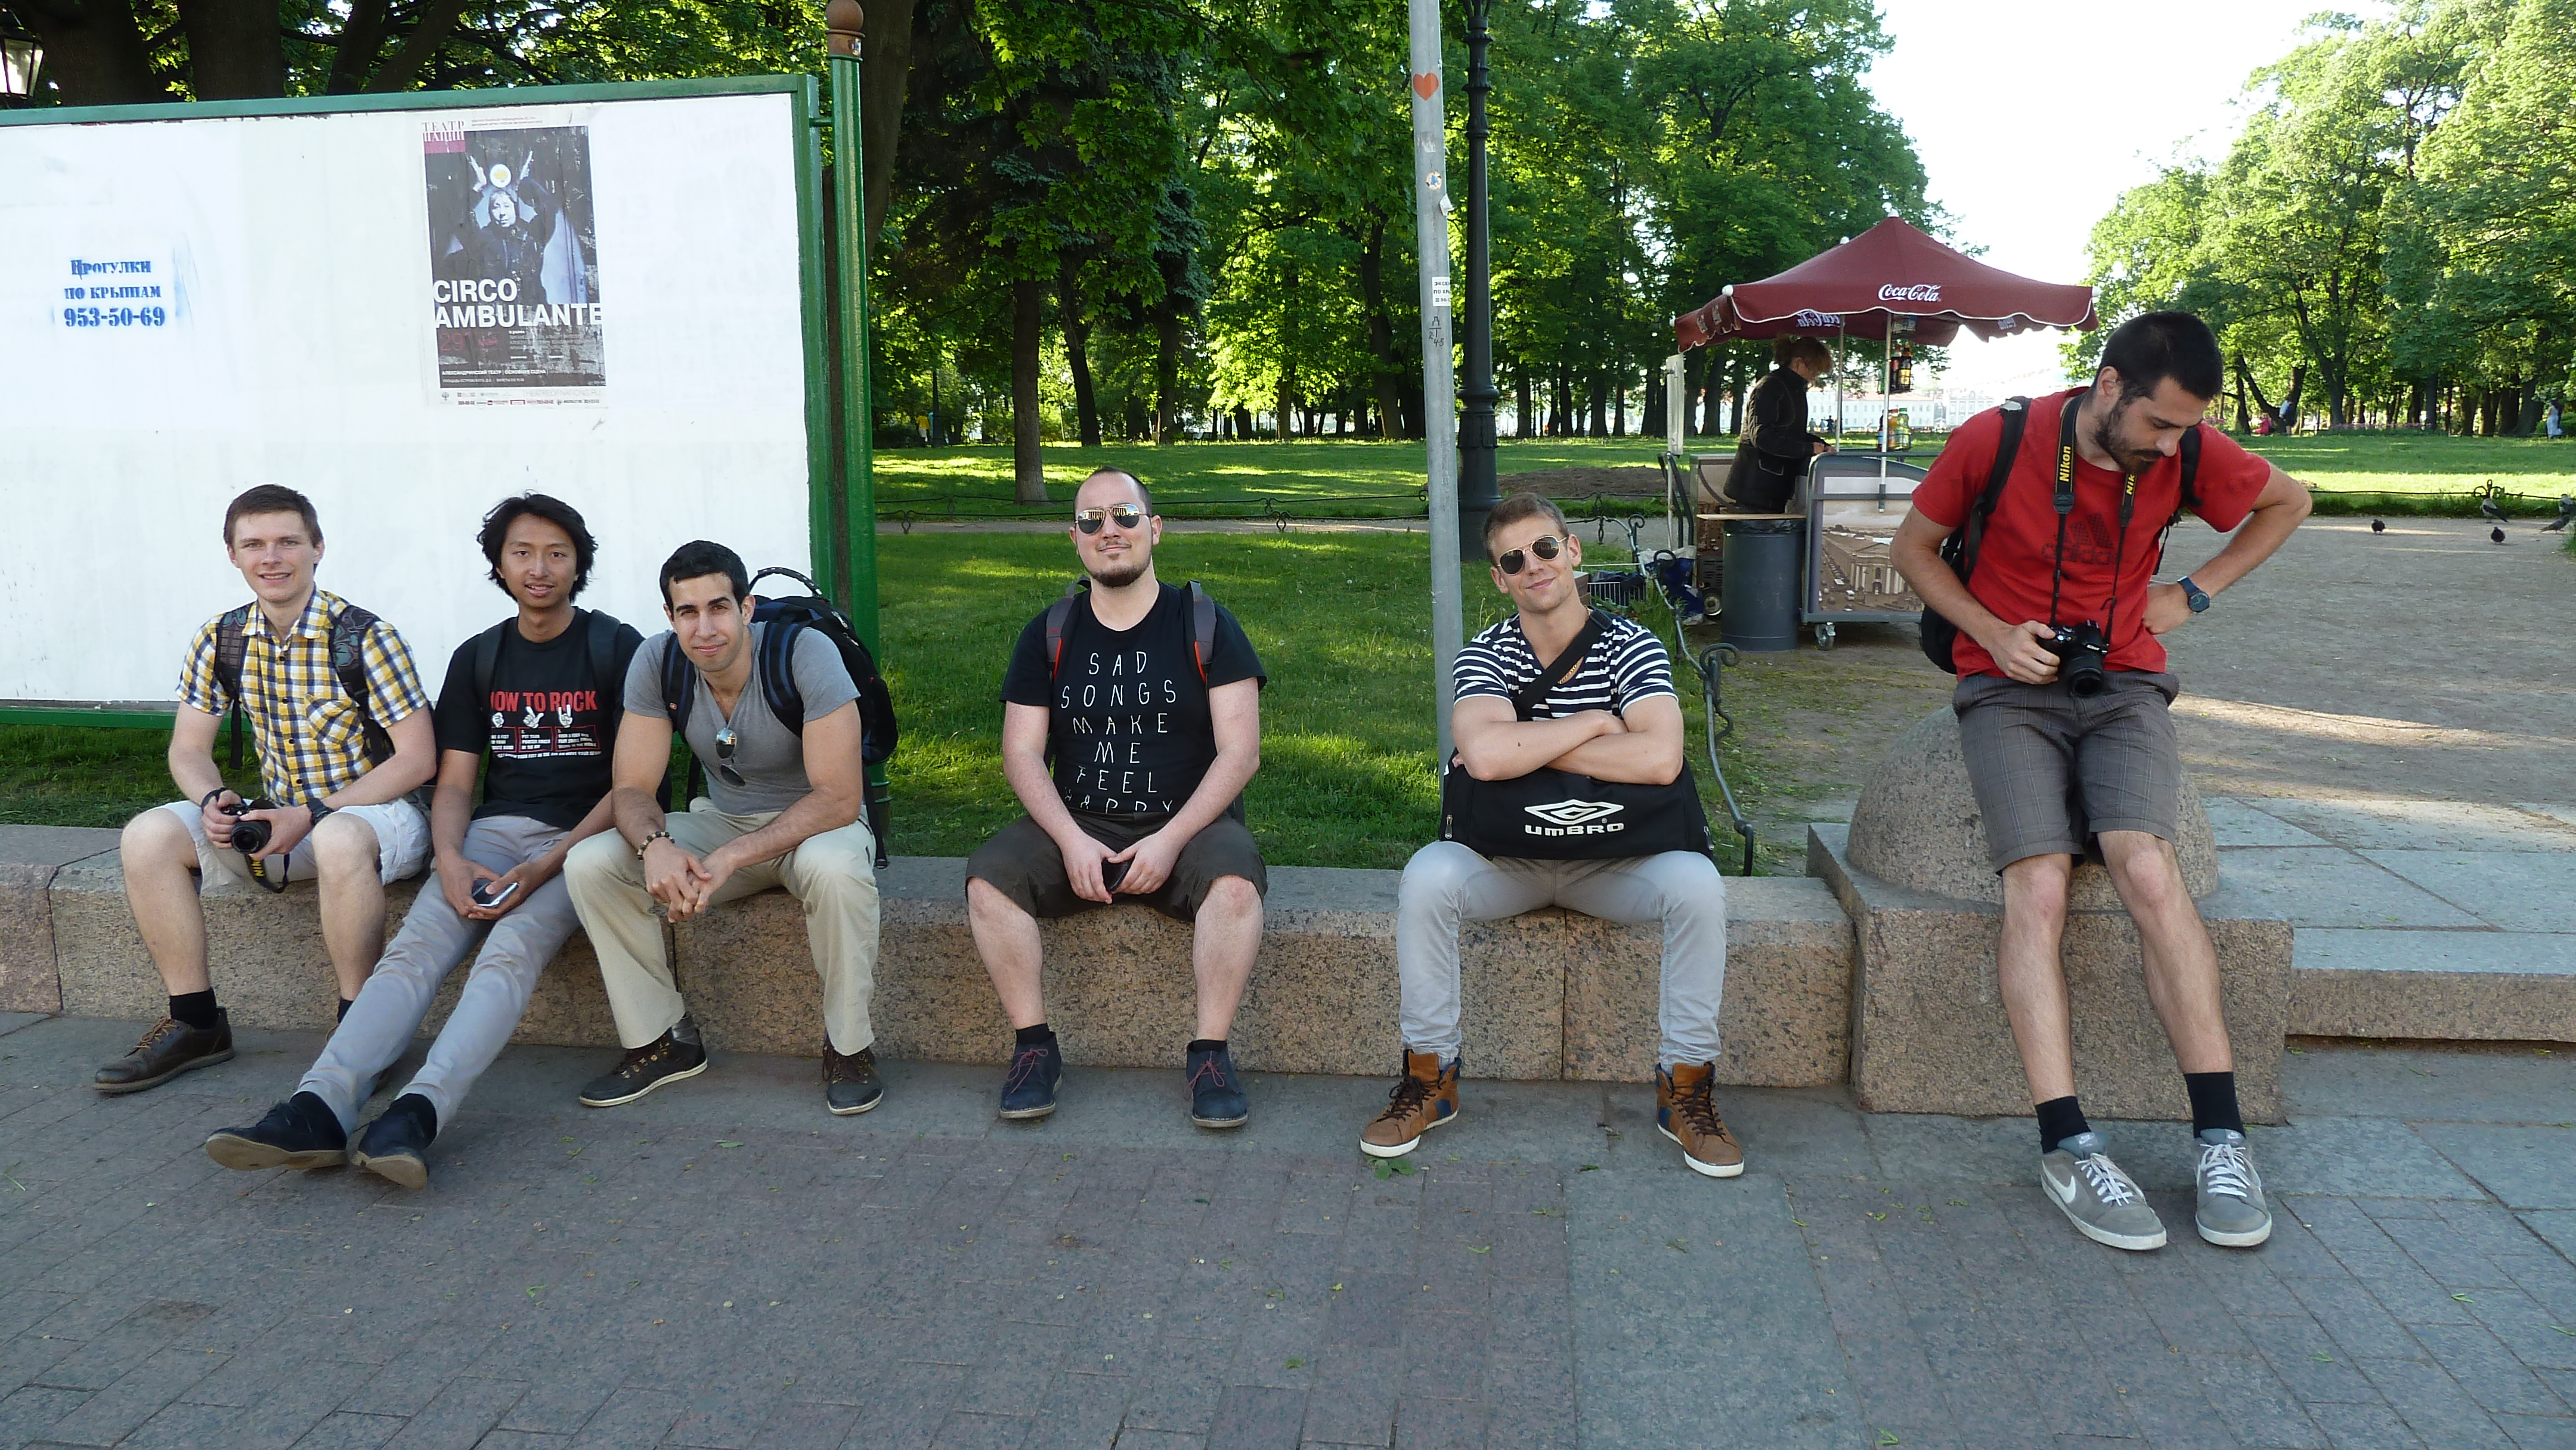
\includegraphics[width=0.5\linewidth]{media/closing_picture.jpg} % Example of an image taking up the total width of the page

	\vspace{10pt}
\end{center}
%----------------------------------------------------------------------------------------

\end{document} 